\chapter{Image processing}
\label{ch:ImageProcessing}
\graphicspath{{Chapter3/Chapter3Figures/}}
The previous chapter focused on existing methods of grading tests automatically. It was found that most systems only use image processing, without a machine learning component, to grade these tests. In this chapter the core techniques behind processing these answer sheets, using image processing, are described. By using only these image processing techniques a reasonably accurate system can already be constructed. For further improvements in accuracy, two machine learning approaches can be implemented.

\section{Orientation detection}
\label{sec:orientDetect}
As mentioned in Section \ref{sec:StandardTech}, there are two main steps in OMR grading. The first challenge with grading a scanned answer sheet, is finding the orientation of the template in the image. This can be done by finding two or more reference points on the page. These reference points then allow for the calculation of the template's rotation, offset and size inside the image. In Chapter \ref{ch:LiteratureStudy} it was found that the traditional way to find these reference points was to include them on the page, in the form of black blocks or lines. Including black blocks is an effective method of finding the template, but might look a bit less attractive, due to the black blocks on the page.

For this project, the markers or reference points that the software uses are already present on the template paper. These are the two longest horizontal lines as well as the two vertical lines on the comment box, as can be seen in Figure \ref{fig:radonResults}. Together, these lines have enough information to determine 4 reference points, shown in red in the figure. These lines are chosen as references, since a Radon transform can easily be applied to locate them, as discussed in Section \ref{sec:RadonTransform}. The system only needs three of those four lines to find the template and thus can successfully find the template even though one of the four lines is identified incorrectly. Using the reference points the rotation, offset and size of the template is determined. However, before the orientation of the image can be determined, a check must be made to determine if the image might be upside down. This is done to make it easier to find the orientation afterwards. To determine if an image is upside down, initial image filtering is required as discussed in the next section.

\begin{figure}
  \centering
  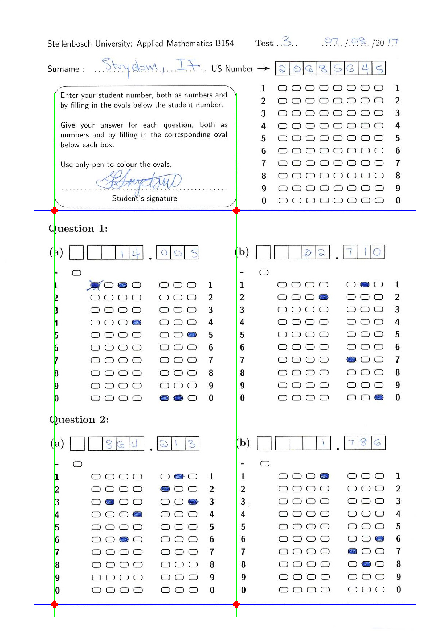
\includegraphics[width=7cm]{RadonResults}\\
  \caption{Four markers found from applying Radon transforms.}
  \label{fig:radonResults}
\end{figure}

\subsection{Initial filtering and orientation detection}
\label{sec:InitImageFilter}

In order to check if an image is upside down, the software first needs to find relevant contours on the page. The contours are then filtered out if it does not loosely match the characteristics of a bubble or character block. This process can be described in Algorithm \ref{alg:checkRot}.

\begin{algorithm}[H]
\caption{: Filter contours and check image rotation.}
\label{alg:checkRot}
\begin{enumerate}
\item Threshold the image by making all the pixel values either white (lower than the mean) or black (higher than the mean).
\item Conduct contour analyses on the image to find all the contours, using the Python library OpenCV.
\item Filter through the contour array to filter out all contours that are not approximately the desired size and aspect ratios.
\item Save these contours for later use.
\item Determine if more contours lie above the middle of the image. This is true if the image is orientated upright. Rotate the image by 180$^{\circ}$ otherwise.
\end{enumerate}
\end{algorithm}

\begin{figure}[h]
  \centering
  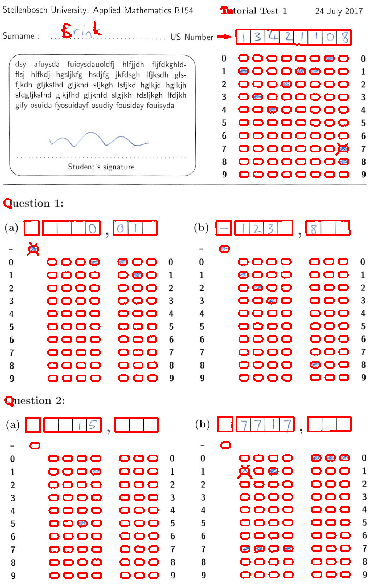
\includegraphics[width=6.5cm]{Reduced}\\
  \caption{Reduced contours in image.}
  \label{fig:reduced}
\end{figure}

It is important to note that there are still unwanted contours in the list, but for now this reduced list is sufficient. Once the list is found, the software counts the number of contour centrepoints below and above the image center. Figure \ref{fig:reduced} shows the resulting contours found in the image. As can be seen in the figure, more bubbles should be below the horizontal center line, for the image to be the right side up. The next step will be to determine the coordinates of the answers the student wrote down, by first locating the template in the image. In the next section a mathematical transform is define, which is used to find the template.

\subsection{Radon transform}
\label{sec:RadonTransform}
\nomenclature[S]{$G(r,\theta)$}{Radon transform defined over $r$ and $\theta$}
\nomenclature[S]{$f(x, y)$}{Two dimensional function that a Radon transform is applied over}
\nomenclature[S]{$x$}{Horizontal coordinate value in two dimensional plane}
\nomenclature[S]{$y$}{Vertical coordinate value in two dimensional plane}
\nomenclature[S]{$r$}{Length of perpendicular offset of the line in a Radon transform}
\nomenclature[S]{$\delta$}{Dirac delta function maps any function to its value at zero}
\nomenclature[S]{$\theta$}{Angle of summation line in the Radon transform}
\nomenclature[S]{$f(x, y)$}{Two dimensional function that a Radon transform is applied over}
\nomenclature[A]{$CT$}{Computed tomography}
\nomenclature[S]{$G_\theta(r)$}{The Randon transform's values at a given $\theta$}
The Radon transform is an integral transform that can be represented by a series of line integrals over a function $f(x,y)$. These transforms are commonly used in Computed Tomography (CT) scans where cross-sectional images of the body are needed. Mathematically this transform is defined as 
\begin{align}
G(r,\theta) = \int_{-\infty}^{\infty} \int_{-\infty}^{\infty} f(x, y) \delta(x\cos(\theta) + y\sin(\theta) - r) dx dy,
\label{eqn:radon}
\end{align}where $r$ represents the perpendicular offset of the line and $\theta$ the angle of the line. The variables $x$ and $y$ specify coordinates in a two-dimensional space within which the function $f(x,y)$ is defined.  A visual interpretation of this transform is shown in Figure \ref{fig:RadonT}. In the figure $G_\theta(r)$ is the Randon transform's values at a given $\theta$.
\begin{figure}[h]
  \centering
  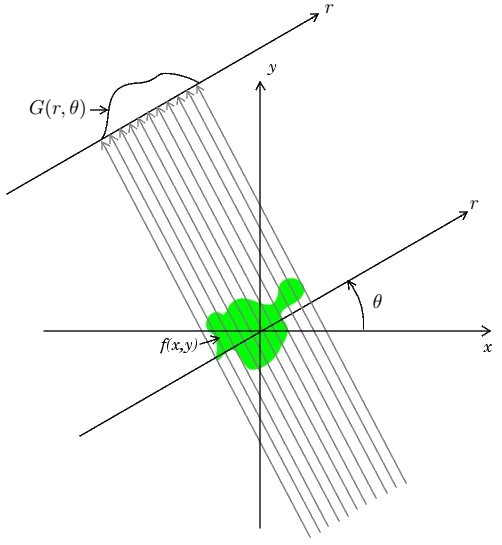
\includegraphics[width=5.6cm]{RadonT}\\
  \caption{Radon transform applied on function $f$, adapted from \citet{radon}.}
  \label{fig:RadonT}
\end{figure}
\subsection{Finding the template}
\label{sec:findTemplate}

In this project, the image's Radon transform is calculated for specific intervals of the gradient. Each gradient interval will thus generate a one dimensional array of values corresponding with the pixel intensities along the lines that are being summed, as shown in Figure \ref{fig:RadonT}. This method is used to determine where the 2 horizontal and 2 vertical lines are located, as previously mentioned.

The Radon transform's values are calculated between the angles 85$^{\circ}$ and 95$^{\circ}$ to find the first two horizontal lines. It is assumed that the image will not be rotated by more than 5$^{\circ}$ in either direction. Black lines will cause a spike in value to appear on the Radon transform for the angle where it is summing parallel with that particular black line. By finding the transform angle that has this spike in value, the rotation of the template can be found. The two maximum values that are recorded at this angle are then taken as the relative locations of the two horizontal lines. After the correct angle is found, the two vertical lines can be found by applying a Radon transform at an angle 90$^{\circ}$ clockwise from the previously calculated angle. The two peak values at that angle then provides the relative locations of the two vertical lines. The four reference points can now be calculated, as seen in Figure \ref{fig:radonResults}. Once the reference points are found, the image is rescaled and orientated to the original template size for further processing. In Figure \ref{fig:rotate} the corrected image is shown.

\begin{figure}
  \centering
  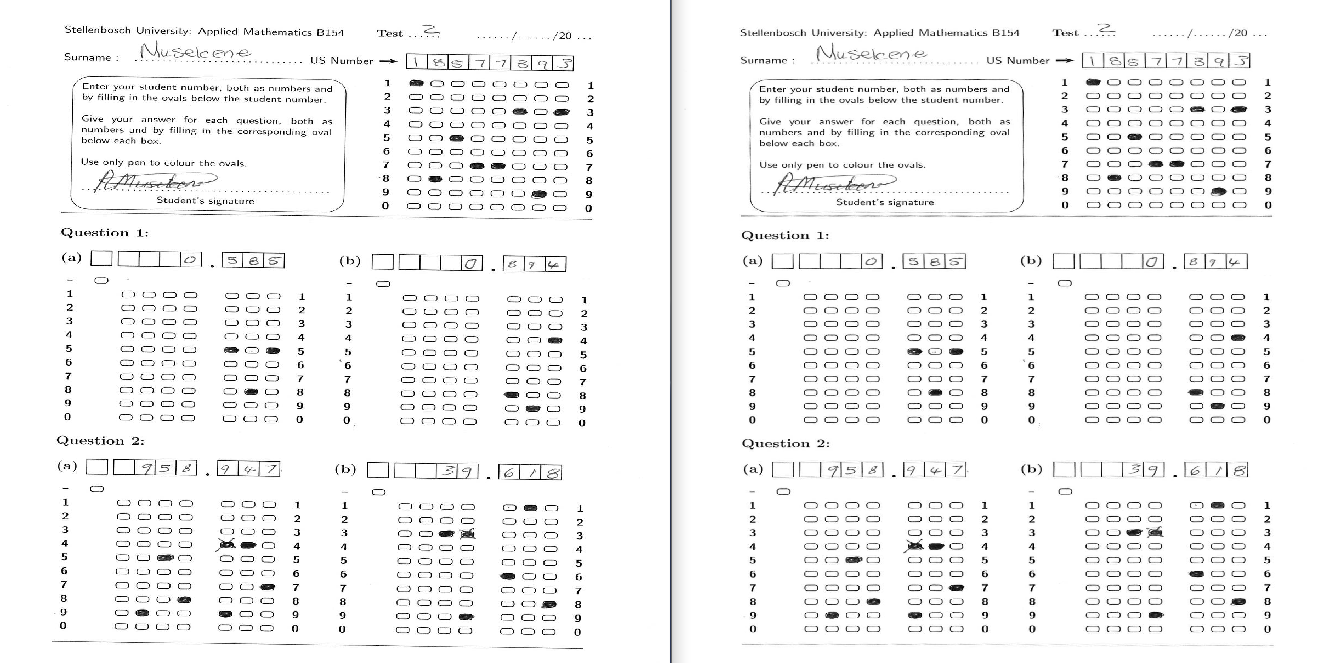
\includegraphics[width=14cm]{Rotation}\\
  \caption{Result in rotation after applying radon transform.}
  \label{fig:rotate}
\end{figure}

Once the template is located the bubble values and digit blocks can be determined, using reference location. These reference locations were calculated in preprocessing conducted on an empty template. Figure \ref{fig:FinalEstimate} illustrates the final estimation of all the bubbles in the template. The estimated bubble centres are coloured red, while the green points represent the centres of all the remaining contours.

\begin{figure}
  \centering
  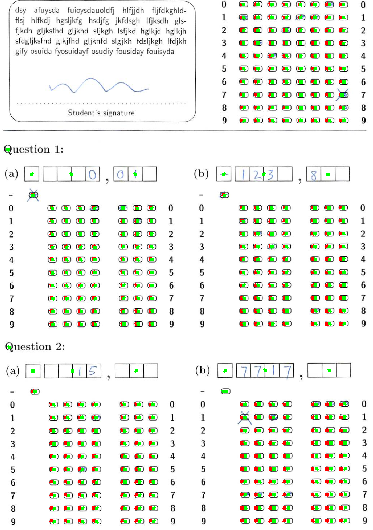
\includegraphics[width=6cm]{FinalEstimate}\\
  \caption{Detection of contours in image and estimation of bubble locations.}
  \label{fig:FinalEstimate}
\end{figure}

Now that a list of possible bubble contours are found with the estimate bubble centres, one contour needs to be assigned to each bubble.

\section{Bubble detection and processing}
\nomenclature[S]{$n$}{Number of bubbles of template sheet}
The location of each bubble in the image is found by simply taking the contour closest to that particular bubble's estimated location. This is done in an efficient manner by sorting the contours by their locations. Searching through the contours now becomes linear and of complexity $O(n)$, where $n$ is the number of bubbles. This means that the processing time to find these bubbles is linearly related to the number of bubbles in the template image. 

Next, the data in each contour needs to be processed and stored. The first type of evidence is obtained from calculating the average pixel intensity inside the contours. If this value is high, the bubble is most likely coloured in or crossed out. The advantage of using the closest contour as the bubble's estimated location, over conventional methods, now becomes apparent. In conventional methods, only pixels at the bubble's estimated location are used to determine if the bubble is coloured-in. This becomes problematic if the system needs to know if the bubble has been crossed out, as the only data available is about pixel intensities. 

Using the contours information about the shape of the bubble entry is also known. Thus by drawing the smallest possible block around the contour, that still covers every value inside the contour, an area can be calculated. This area becomes large when a answer is crossed out, due to the lines stretching outside the initial bubble. By inspecting the area value, the system can successfully determine if the bubble is filled in or crossed out.

\section{Data processing and grading}

The previous section now allows each bubble to be classified into three categories namely, empty, completely filled-in or crossed out. An additional category of partially filled in is also introduced, as it aids grading of tests where students write lightly. An algorithm to determine what bubble was chosen is described in Algorithm \ref{alg:bubbleAns}.

\begin{algorithm}[H]
\caption{: Calculate the student answer from bubble grid.}
\label{alg:bubbleAns}
\begin{enumerate}
\item Start with column 0.
\item Count the number of completely filled-in answers in this column. Store the position of that entry for later use.
\item If there are no completely filled-in answers, count the amount of partially filled-in answers and override the previous values.
\item If the previous result is 0, set the output value for that column to 0.
\item If step 2 or 3 presents a value greater that 1, save the answer sheet to a clash list to be evaluated manually once the automatic grading of the test is completed.
\item Repeat steps 2 to 5 for each column in the bubble grid.
\end{enumerate}
\end{algorithm}



This algorithm therefore checks if there are more that one entry in any of the columns. If this is true, the results are sent to a clash list to be marked manually. If one bubble was found to be coloured in, the value gets set to the index of that bubble. Finally, if no bubbles where coloured in the result for that column are set to 0.

\section{Conclusion}

This chapter provided an overview of a basic automatic test grading system using image processing and computer vision. The system can achieve acceptable results using only these techniques.

The following chapter will focus on applying additional machine learning techniques to further improve the accuracy of grading these tests.